
\documentclass{ctexart}

\author{李约瀚 \\ 14130140331 \\ qinka@live.com \\ qinka@qinka.pw}
\title{FPGA设计基础实验报告 (三)}

\usepackage{listings}
\usepackage[figuresright]{rotating}
\lstset{breaklines}

\begin{document}
    
        % Cover
        \thispagestyle{empty}
        \begin{center}
            \vspace*{4em}
            {\Huge\textbf{FPGA设计基础实验报告\\\vspace*{0.5em} (三)}}
            \vfill
            \large
            \begin{tabular}{c@{:}l}
                班级 & 1413014 \\
                学号 & 14130140331 \\ 
                姓名 & 李约瀚 \\ 
                教师 & 沈沛意 \\
            \end{tabular} 
            \vspace*{4em}\\
        \end{center}
        \newpage
        
       
        % Setting
        \setcounter{page}{0}
        \setcounter{section}{0}
        %\renewcommand\thesection{实验编号 1-\numeric{section} 题目: }
        %\renewcommand\thesubsection{}
        %\renewcommand\thesubsubsection{(\numeric{subsubsection})}

        % Exp 3-1

        \section{Xilinx 嵌入式下系统设计(I)}
        
        \subsection{实验目的}
        \begin{itemize}
            \item 了解 FPGA 嵌入式系统的设计基本概念与特点
            \item 了解 MicroBlaze, 与对应的外设
            \item 了解 EDK 开发的基本流程
        \end{itemize}
        
        \subsection{实验步骤}
        
        \begin{itemize}
            \item 简单的硬件设计
            \item 添加 IP 核到硬件设计
            \item 配置 SDK
            \item 编写软件
            \item 配置上板
        \end{itemize}

        \subsection{预备知识}
        
        \subsubsection{EDK 开发流程}
        
        \begin{enumerate}
            \item 在 XPS 中开发嵌入式硬件
            \begin{itemize}
                \item 使用 Base System Builder 针对目标板快速开发系统
                \item 利用 IP 核 添加外设,扩展系统
                \item 使用 PlatGen 生成 HDL 网表
            \end{itemize}
            \item 在 SDK 中开发嵌入式软件
            \begin{itemize}
                \item 使用 LibGen 生成库和驱动
                \item 使用 SDK 开发与调试
                \item 使用 XMD 与 GDB 调试软件。
            \end{itemize}
            \item 生成配置
            \begin{itemize}
                \item 生成比特流使用 iMPACT 配置 FPGA 芯片
            \end{itemize}
            \item 部署
            \begin{itemize}
                \item 使用 Flash Writer utility 初始化外部闪存,从闪存中启动系统;或者使用 System ACE File Generator 生成外部 CF 卡配置文件,并从 CF 卡启动。
            \end{itemize}
        \end{enumerate}
        
        \subsection{实验内容}
        
        \subsubsection{系统结构与设计}
        
        完整的系统设计如图 \ref{fig:report3-1} 所示,其中
        本次实验的设计内容如图 \ref{fig:report3-2} 所示。
                
        \begin{figure}[h!]
\centering
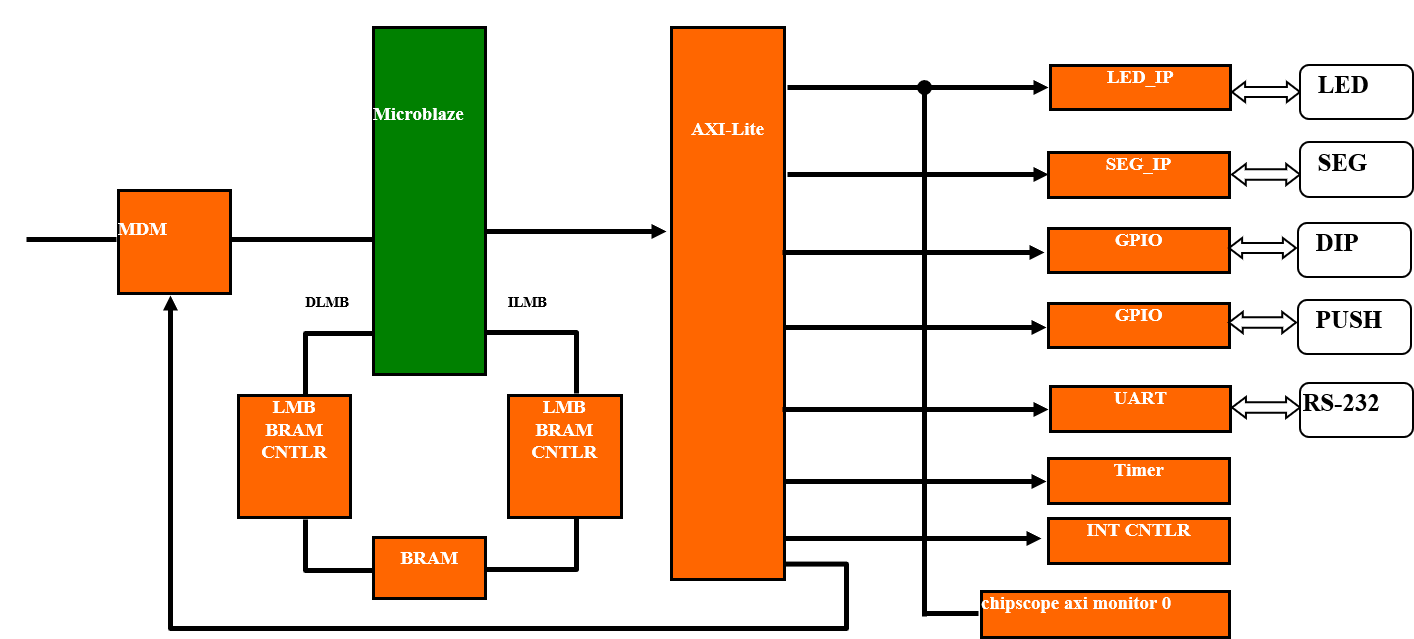
\includegraphics[width=1\linewidth]{report3-1}
\caption{系统完整结构}
\label{fig:report3-1}
        \end{figure}
        
        \begin{figure}[h!]
\centering
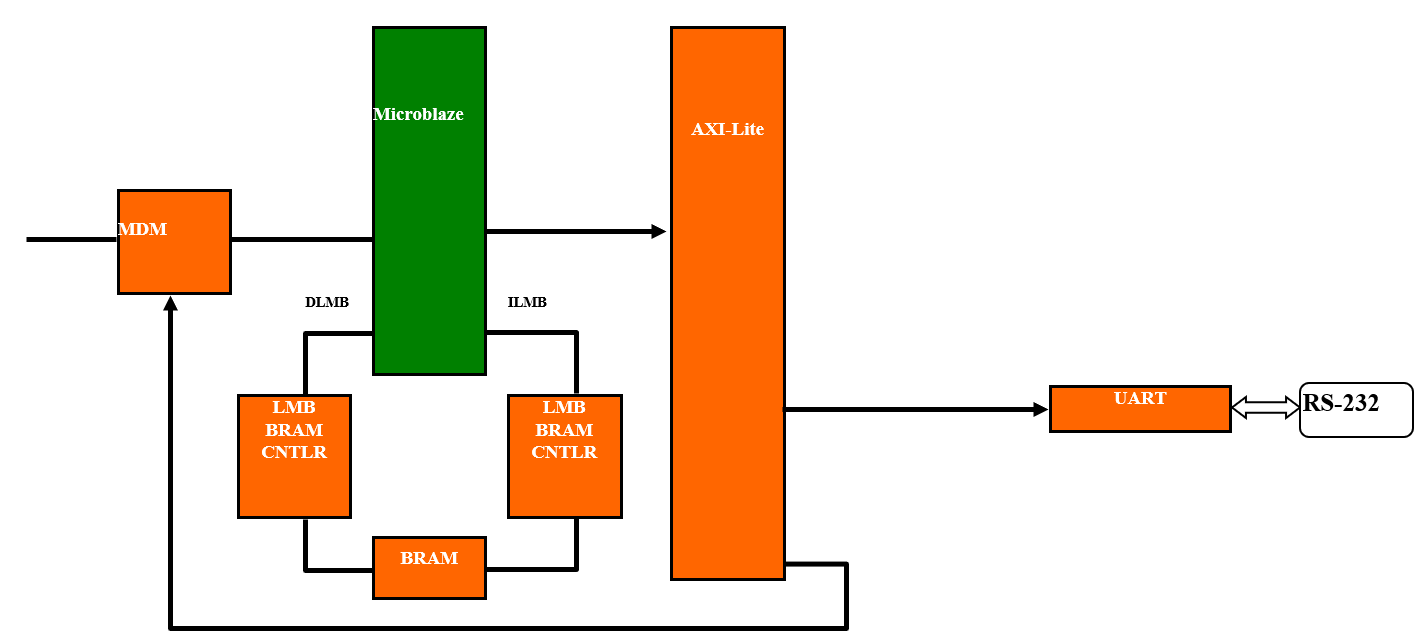
\includegraphics[width=1\linewidth]{report3-2}
\caption{实验内容}
\label{fig:report3-2}
        \end{figure}
        
        \paragraph{新建工程}
        
        在 XPS 通过 “Create New Project Using Base System Builer” 创建新的项目。
        
        在一个完整的路径中创建一个基于 AXI System 的系统。
        在提前安装好对 Digilent 的 Nexys 3 的板级支持包之后,
        配置我们的开发板。
        
        将 \verb|Local Memory Size| 设置为 16KB,
        并将除串口通信以外的所有外设移除。并点击 Finish
        结束向导。
        
        \subsubsection{添加 IP 核}
        
        由于本实验未设置其他内容,故不需要添加 IP 核。
        
        \subsubsection{配置 SDK}
        
        在正式配置 SDK 之前,需要依次通过 
        \verb|Generate Netlist| 与 \verb|Generate Bitstream|
        生成网表与比特流文件。
        
        然后在 \verb|Project -> Export Hardware ...| 选项中
        到处对于硬件的设计支持的 SDK。
        在弹出的对话框中,选择 \verb|Export \& Launch SDK|,
        并在 SDK 打开之后将工作空间定位到工程中的
        \verb|SDK\SDK_Export| 目录下。
        
        然后在 \verb|File -> New| 菜单选项中选择 \verb|Other|
        然后在对话框中找见 \verb|Board Support Package|
        创建板级支持包。

        然后在向导中选择 \verb|standalone| 并创建板级支持包。
        然后还是在 \verb|File -> New| 菜单中选择 \verb|Application|
        创建 C语言 的 HelloWorld 工程,并选择之前创建的板级支持包。
        
        \subsubsection{编写软件}
        
        我们的 \verb|Hello World| 跨越过一堆坑之后,终于可以开始编写了。
        在代码中编写:
        
        \begin{lstlisting}[language=C,caption=]
#include <stdio.h>
#include "platform.h"

void print(char *str);

int main()
{
    init_platform();

    print("Hello World\n\r");
    print("I was created on an unsuspecting world.\n\r");
    cleanup_platform();

    return 0;
}
        \end{lstlisting}

        \subsubsection{配置上板}
        
        在代码保存之后,程序是自动编译的,因此至此所需要的文件基本都准备好了。
        
        \paragraph{链接串口}
        
        在之前设计硬件的部分是使用串口进行通信。在 Windows 上使用
        PuTTY这个软件进行与 FPGA 开发板的通行。对于 macOS 或者 Linux
        等 Unix类的系统则是使用 minicon 进行串口的链接。
        
        之前配置的是 波特率是 115200,则在配置中配置好。
        
        然后在JTAG 配置中,配置成 Diligent 的 USB。然后将之前生成好的文件通过
        \verb|Xilinx Tools -> Program FPGA|  中的选项配置好的比特流文件与生成的可执行的ELF文件,将其刷入 FPGA中。

        然后在串口链接工具中可以看见输出的内容,如图\ref{fig:report3-4}所示。

\begin{figure}
\centering
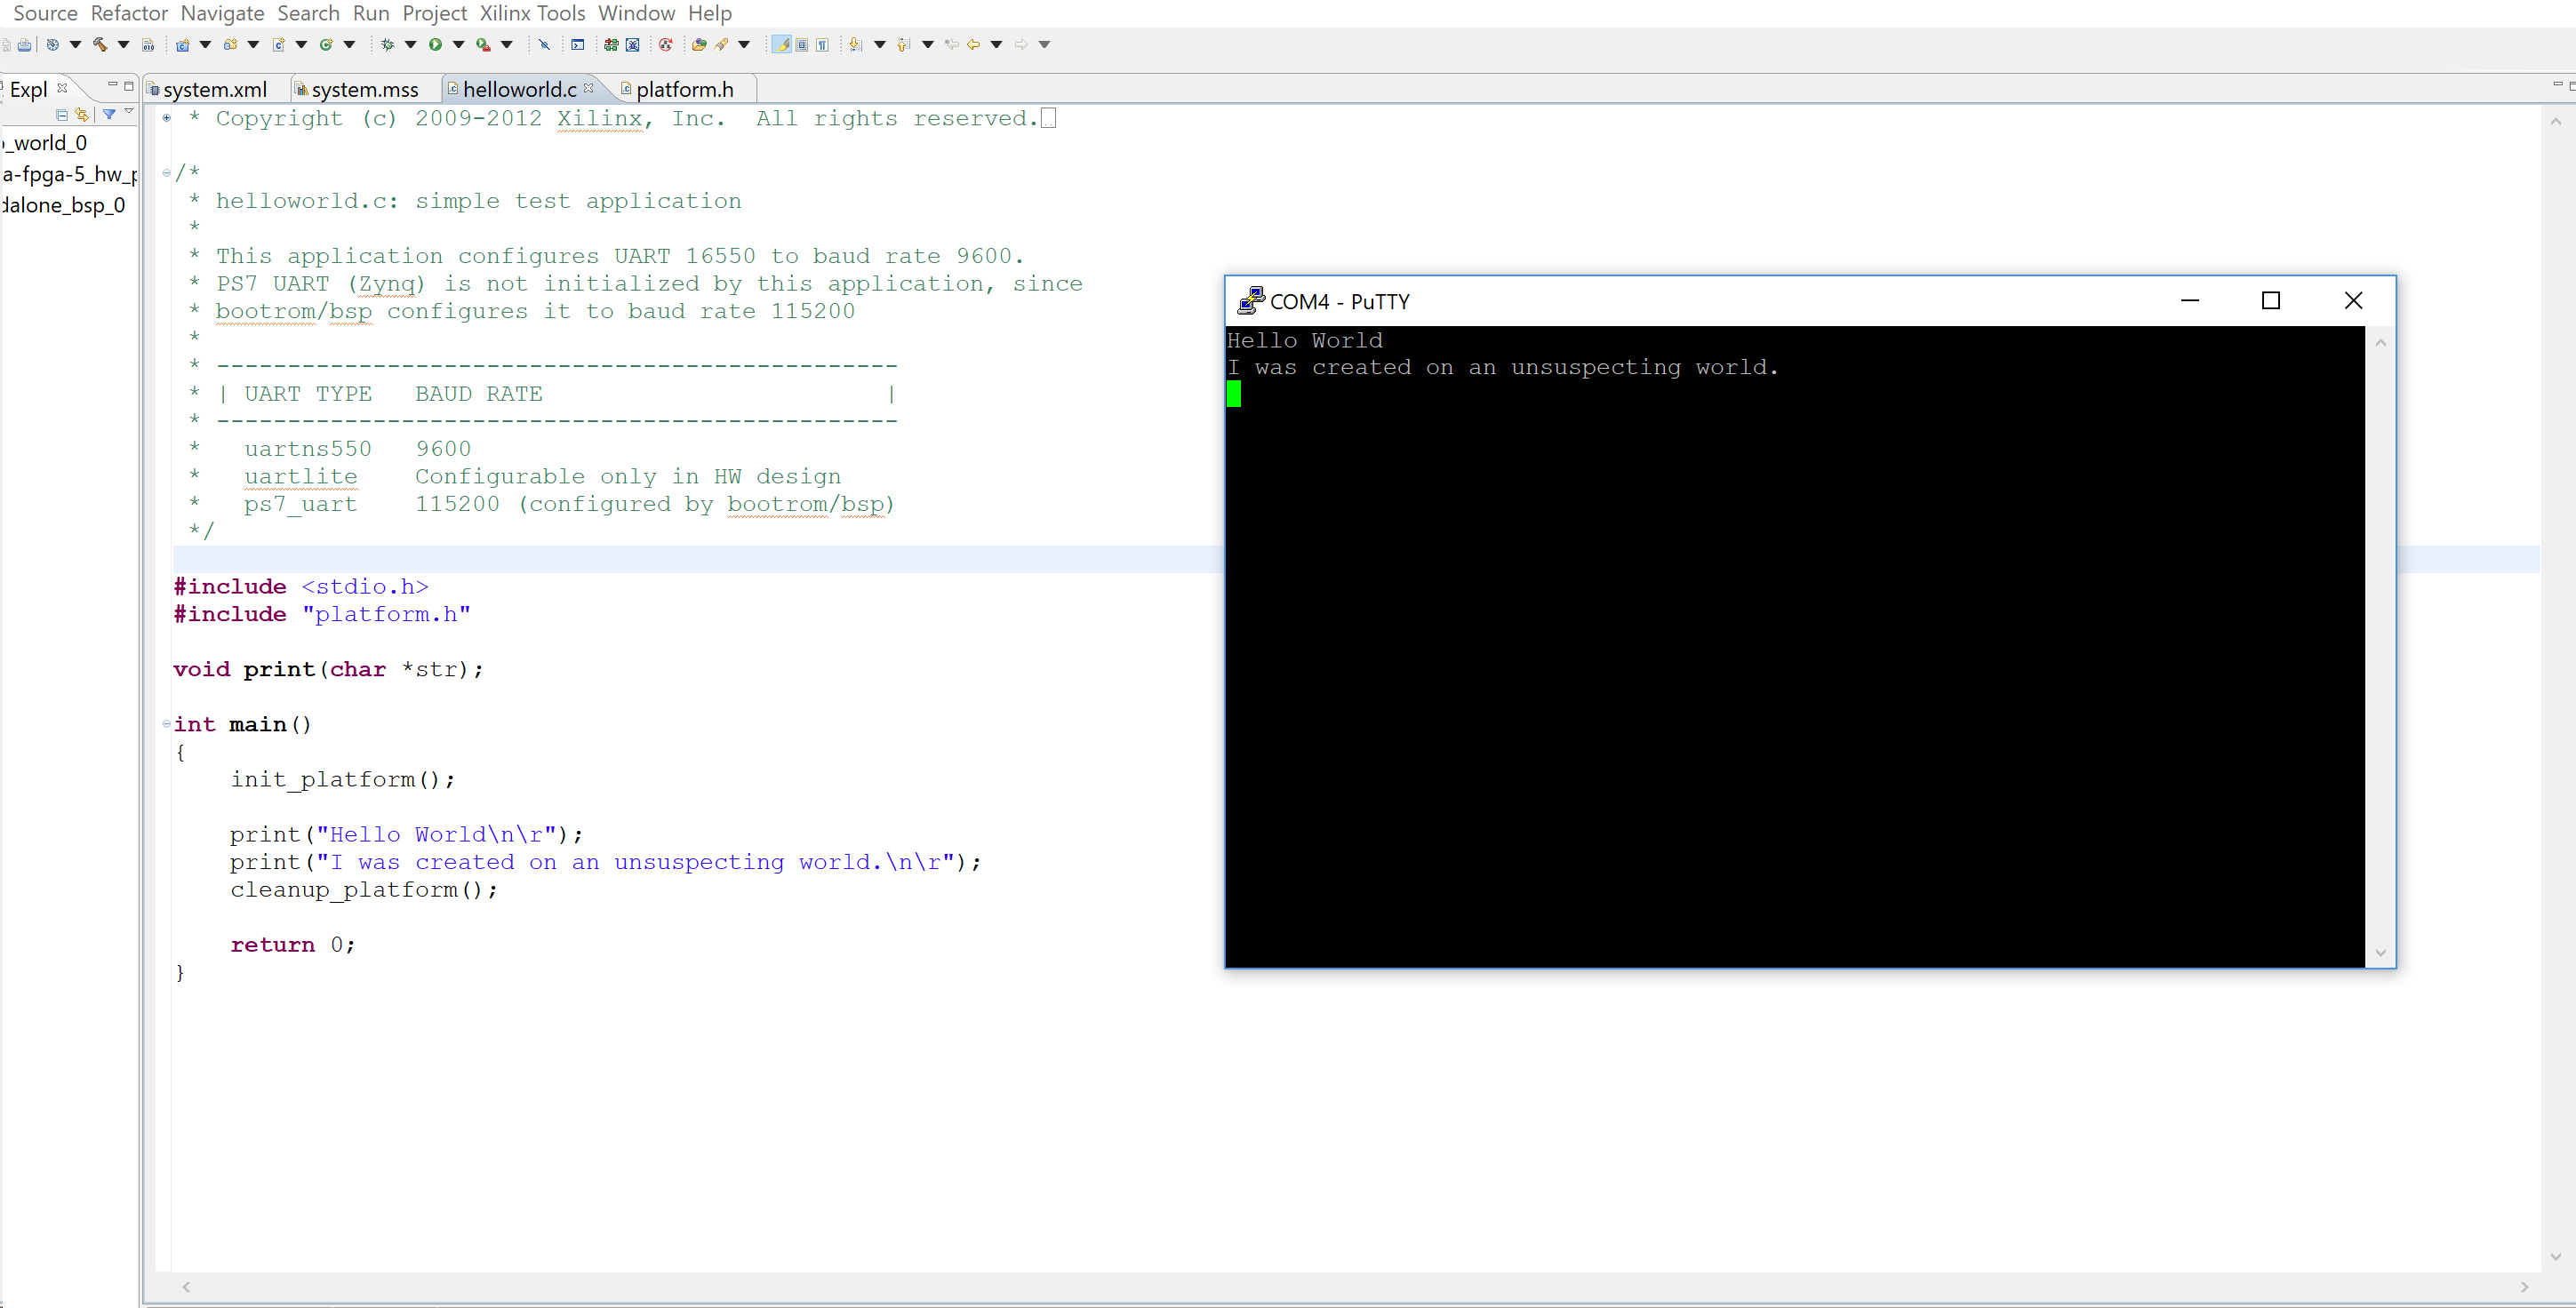
\includegraphics[width=1\linewidth]{report3-4}
\caption{输出结果}
\label{fig:report3-4}
\end{figure}


        % Exp 3-2

        \section{Xilinx 嵌入式下系统设计(II)}
        
        \subsection{实验目的}
        \begin{itemize}
            \item 了解 FPGA 嵌入式系统的设计基本概念与特点
            \item 了解 MicroBlaze, 与对应的外设
            \item 了解 EDK 开发的基本流程
        \end{itemize}
        
        \subsection{实验步骤}
        
        \begin{itemize}
            \item 简单的硬件设计
            \item 添加 IP 核到硬件设计
            \item 配置 SDK
            \item 编写软件
            \item 配置上板
        \end{itemize}

        \subsection{实验内容}

        \subsubsection{系统结构与设计}

        系统完整的设计如图 \ref{fig:report3-1} 所示,其中本次实验的
        设计内容如图 \ref{fig:report3-3} 所示。
      
        \begin{figure}[h!]
          \centering
          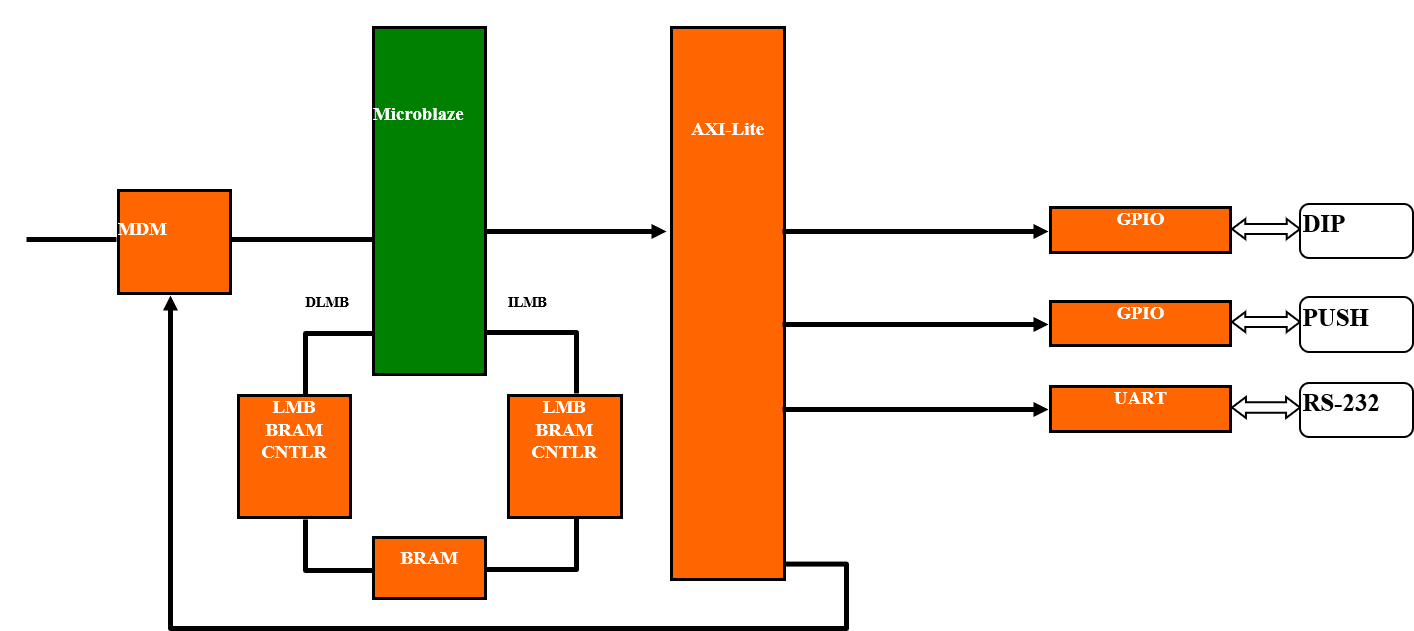
\includegraphics[width=1\linewidth]{report3-3}
          \caption{本次实验的内容}
          \label{fig:report3-3}
        \end{figure}
        
        \paragraph{新建工程}
        
        在 XPS 通过 “Create New Project Using Base System Builer” 创建新的项目。
        
        在一个完整的路径中创建一个基于 AXI System 的系统。
        在提前安装好对 Digilent 的 Nexys 3 的板级支持包之后,
        配置我们的开发板。
        
        将 \verb|Local Memory Size| 设置为 16KB,
        并将除串口通信以外的所有外设移除。并点击 Finish
        结束向导。
        
        \subsubsection{添加 IP 核}

        点击 \verb|IP Catalog| 标签,在 \verb|General Purpose IO| 下选择
        \verb|AXI General Purpose IO|,双击添加 IP 核。一共需要添加两个。
        并设置自动为 IP 核添加链接。并将两个 IP 核改名为 DIP 与 PUSH。

        保持默认配置。并将 PUSH 的 \verb|GPIO Data Channel Width| 配置为 4,
        然后将 \verb|Channel 1 is Input Only| 选中。并通过同样的方式配置 DIP
        实例。其中唯一不同的地方是数据总线的宽度为 8 位。

        点击 \verb|Ports| 标签,查看 DIP 与 PUSH 实例的端口链接。
        删除两者 \verb|GPIO_IO| 端口的链接。并将 两者的 GPIO\_IO\_I 端口设置为外部端口。
        其中需要注意的是需要将 两个的端口的 \verb|Range| 属性设置成对应的 
        $[7:0]$ 与 $[3:0]$。

        最后将大概 154 行与167行的
        \lstinline|PORT GPIO_IO = axi_gpio 0 GPIO_IO| 与
        \lstinline|PORT GPIO_IO = axi_gpio_1 GPIO_IO| 删除。

        然后在 \verb|Project| 标签中双击打开 \verb|system.ucf| 
        添加如下代码:
        
\begin{lstlisting}
#
# pin constraints
#
NET GCLK LOC = "V10"  |  IOSTANDARD = "LVCMOS33";
NET RESET LOC = "B8"  |  IOSTANDARD = "LVCMOS33"  |  TIG;
NET RS232_Uart_1_sin LOC = "N17"  |  IOSTANDARD = "LVCMOS33";
NET RS232_Uart_1_sout LOC = "N18"  |  IOSTANDARD = "LVCMOS33";
#
# additional constraints
#

NET "GCLK" TNM_NET = sys_clk_pin;
TIMESPEC TS_sys_clk_pin = PERIOD sys_clk_pin 100000 kHz;

## Switches
Net "DIP_GPIO_IO_I_pin<0>" LOC = T10 | IOSTANDARD = LVCMOS33;
Net "DIP_GPIO_IO_I_pin<1>" LOC = T9 | IOSTANDARD = LVCMOS33;
Net "DIP_GPIO_IO_I_pin<2>" LOC = V9 | IOSTANDARD = LVCMOS33;
Net "DIP_GPIO_IO_I_pin<3>" LOC = M8 | IOSTANDARD = LVCMOS33;
Net "DIP_GPIO_IO_I_pin<4>" LOC = N8 | IOSTANDARD = LVCMOS33;
Net "DIP_GPIO_IO_I_pin<5>" LOC = U8 | IOSTANDARD = LVCMOS33;
Net "DIP_GPIO_IO_I_pin<6>" LOC = V8 | IOSTANDARD = LVCMOS33;
Net "DIP_GPIO_IO_I_pin<7>" LOC = T5 | IOSTANDARD = LVCMOS33;

## Buttons
Net "PUSH_GPIO_IO_I_pin<0>" LOC = A8 | IOSTANDARD = LVCMOS33;
Net "PUSH_GPIO_IO_I_pin<1>" LOC = C4 | IOSTANDARD = LVCMOS33;
Net "PUSH_GPIO_IO_I_pin<2>" LOC = C9 | IOSTANDARD = LVCMOS33; 
Net "PUSH_GPIO_IO_I_pin<3>" LOC = D9 | IOSTANDARD = LVCMOS33;
\end{lstlisting}

        \subsubsection{配置SDK}
        
        在正式配置 SDK 之前,需要依次通过 
        \verb|Generate Netlist| 与 \verb|Generate Bitstream|
        生成网表与比特流文件。
        
        然后在 \verb|Project -> Export Hardware ...| 选项中
        到处对于硬件的设计支持的 SDK。
        在弹出的对话框中,选择 \verb|Export \& Launch SDK|,
        并在 SDK 打开之后将工作空间定位到工程中的
        \verb|SDK\SDK_Export| 目录下。
        
        然后在 \verb|File -> New| 菜单选项中选择 \verb|Other|
        然后在对话框中找见 \verb|Board Support Package|
        创建板级支持包。

        然后在向导中选择 \verb|standalone| 并创建板级支持包。
        然后还是在 \verb|File -> New| 菜单中选择 \verb|Application|
        创建 C语言 的 Empty Application 工程,并选择之前创建的板级支持包。

        \subsubsection{编写软件}

        然后导入 如下代码
\begin{lstlisting}[language=C]
#include "xparameters.h"
#include "xgpio.h"
#include "xutil.h"
  

//====================================================

int main (void) 
{

   XGpio dip, push;
	int i, psb_check, dip_check;
	
   //xil_printf("-- Start of the Program --\r\n");
 
   XGpio_Initialize(&dip, XPAR_DIP_DEVICE_ID);
	XGpio_SetDataDirection(&dip, 1, 0xffffffff);
	
	XGpio_Initialize(&push, XPAR_PUSH_DEVICE_ID);
	XGpio_SetDataDirection(&push, 1, 0xffffffff);
	
	while (1)
	{
	  psb_check = XGpio_DiscreteRead(&push, 1);
	  xil_printf("Push Buttons Status %x\r\n", psb_check);
	  dip_check = XGpio_DiscreteRead(&dip, 1);
	  xil_printf("DIP Switch Status %x\r\n", dip_check);
	  
	  for (i=0; i<999999; i++); 
	}
 
}
\end{lstlisting}
        
        \subsubsection{配置上板}
        
        在代码保存之后,程序是自动编译的,因此至此所需要的文件基本都准备好了。
        
        \paragraph{链接串口}
        
        在之前设计硬件的部分是使用串口进行通信。在 Windows 上使用
        PuTTY这个软件进行与 FPGA 开发板的通行。对于 macOS 或者 Linux
        等 Unix类的系统则是使用 minicon 进行串口的链接。
        
        之前配置的是 波特率是 115200,则在配置中配置好。
        
        然后在JTAG 配置中,配置成 Diligent 的 USB。然后将之前生成好的文件通过
        \verb|Xilinx Tools -> Program FPGA|  中的选项配置好的比特流文件与生成的可执行的ELF文件,将其刷入 FPGA中。

        然后在串口链接工具中可以看见输出的内容。
        
        \begin{figure}
\centering
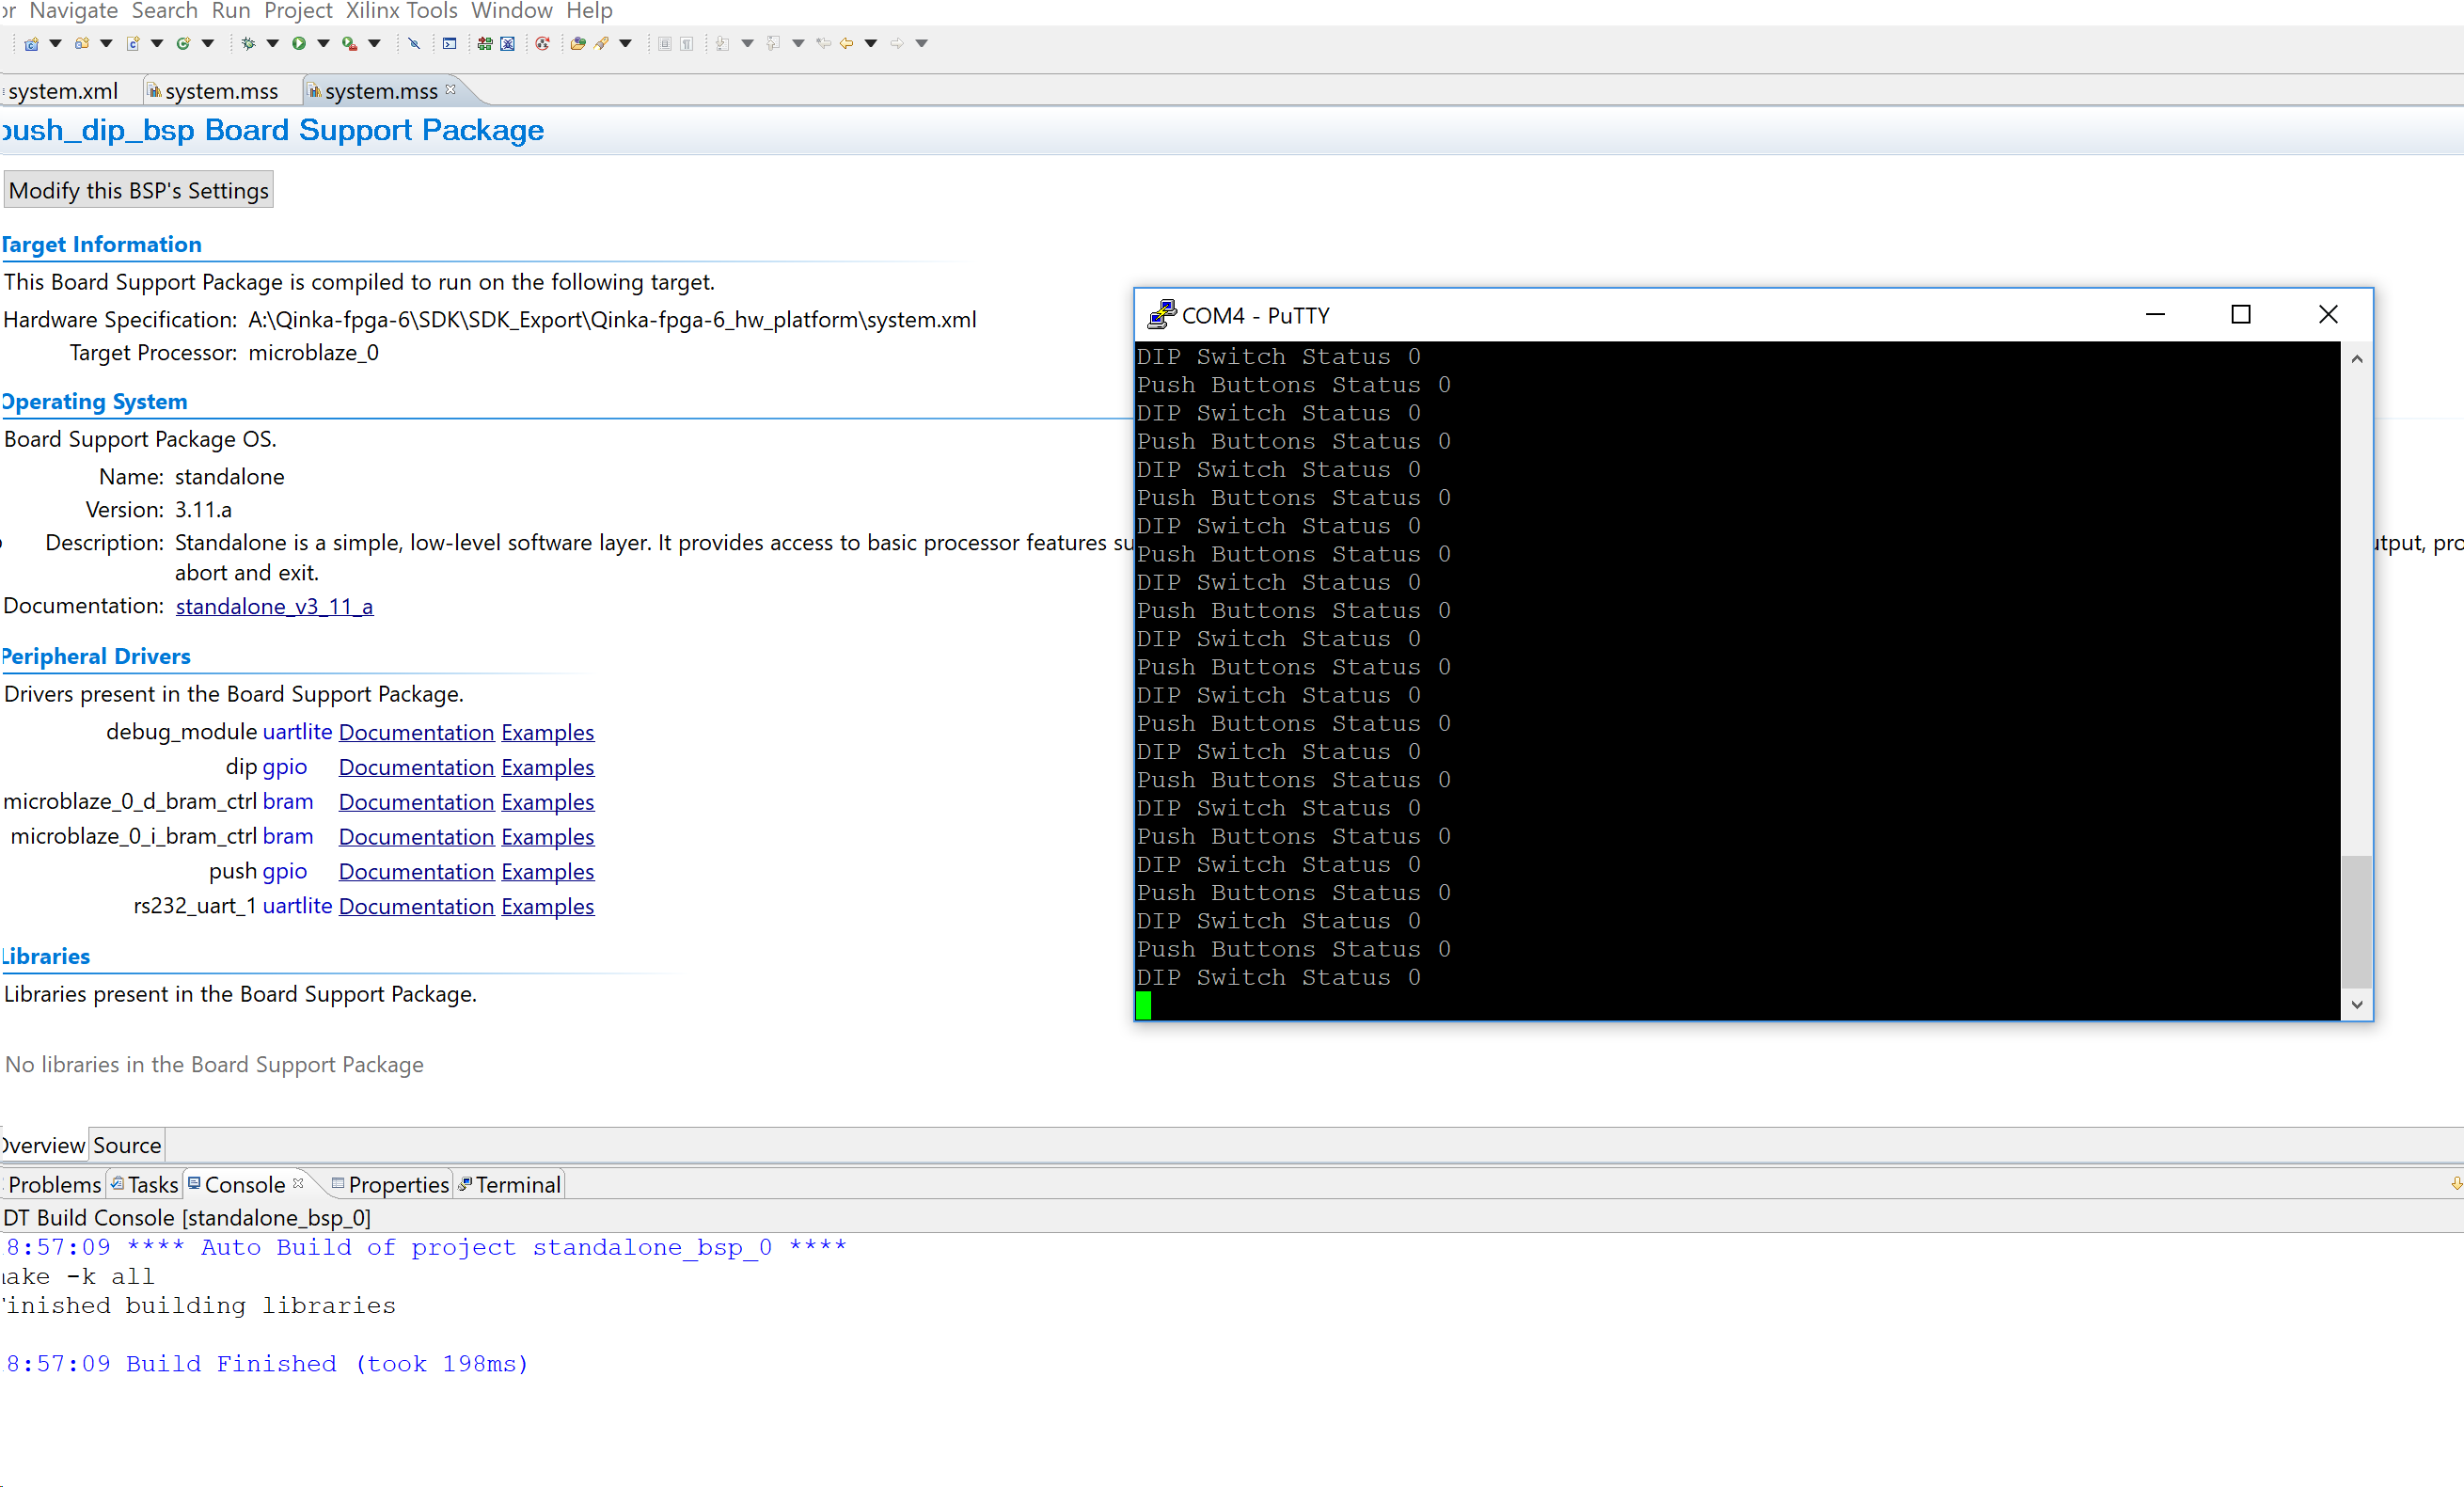
\includegraphics[width=1\linewidth]{report3-5}
\caption{输出结果}
\label{fig:report3-5}
\end{figure}

        



        
\end{document}